\subsection{Definition af overbelægning}
Overbelægning opstår, når der er flere patienter på en afdeling end den er normeret til.\cite{Heidmann2014} Dette sker ved akut indtag af uafviselige patienter, hvorved antallet af patienter overstiger antallet af sengepladser. 
Når alle sengepladser på en afdeling er optaget er kapaciteten på $100~\%$. Overbelægning estimeres derfor som en kapacitet på over $100~\%$.

I perioden fra år $1996$ til $2011$ er sengepladserne på de danske hospitalsafdelinger reduceret med $30~\%$, hvilket har forårsaget at antallet af disponible senge er reduceret. Dette kan få en betydning for antallet af akutte indlæggelser.\cite{Madsen2014}

Antallet af akutte indlæggelser varierer hver måned, hvorfor tilgængeligheden af sengepladser ligeledes variere. Det fremgår af \figref{overbelaegning_ran}, at overbelægning opstår på flere hospitalsafdelinger i Danmark. Ud af de $50$ tilfældige hospitalsafdelinger har $35$ svarede til $70~\%$ af afdelingerne oplevet overbelægning i januar måned. Herudover fremgår det af figuren, at nogle afdelinger har haft en belægning på over $100~\%$ op til $31$ dage, hvilket svarer til, at afdelingen har haft overbelægning alle dage i januar måned.\cite{SDS2015}

\begin{figure}[H]
	\flushleft 
	\caption{Overbelægning på $50$ tilfældige hospitalsafdelinger i Danmark}
	\centering
	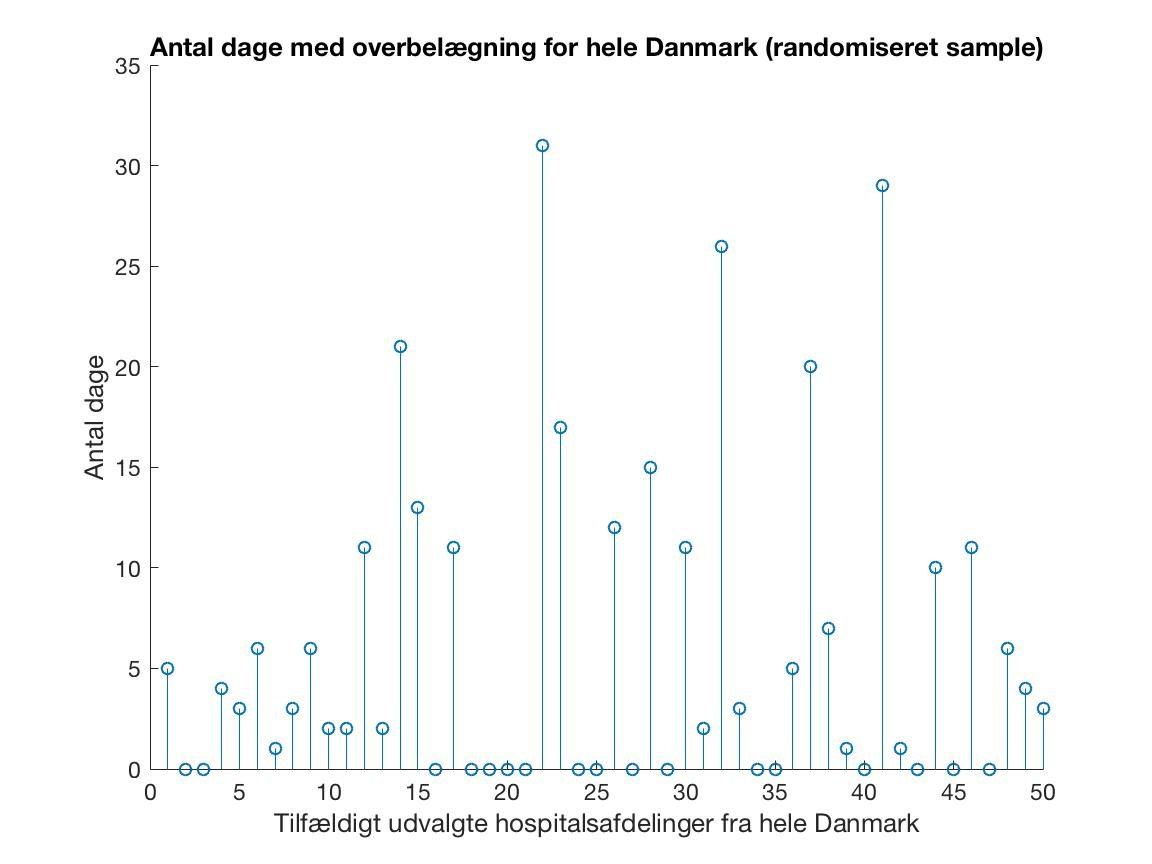
\includegraphics[scale=.3]{figures/overbelaegning_ran}
	\label{overbelaegning_ran}
	\flushleft
	\textit{Illustrerer antal dage med overbelægning på $50$ tilfældige hospitalsafdelinger fra hele Danmark. De tilfældige data er taget fra januar måned år $2015$. \cite{SDS2015}}
\end{figure}

\subsubsection{Omstrukturering af Aalborg Universitetshospital} \fxnote{måske en anden overskrift}
\noindent
Gennem de seneste år er Aalborg universitetshospitals opgave som akuthospital vokset, hvilket har resulteret i at patienttallet udfordrer de disponible sengepladser. Hertil har hospitalet i år $2016$ haft fornyet fokus på at arbejde med sikkert patientflow samt at udnytte senge og ambulatorier effektivt for at patienter og personale skal undgå at opleve overbelægning samt for at undgå flaskehalse. Målet er at minimere patienternes ventetid, undgå unødige inlæggelser samt ambulante besøg. \cite{Handleplan2016}. 

\noindent
I budgetfordelingen for Aalborg Universitetshospital i år $2017$ indgår det, at ventetiden på en operation for elektive patienter skal reduceres fra $57$ dage til $50$ dage.\cite{Budget2016} Dette betyder optimering af planlægning ift. kapacitet. Dette skal ligeledes skabe et mere sammenhængende patientforløb og give bedre patientflow. Hertil kræves det, at tilgængelige ressourcer anvendes mest effektivt.\cite{Handleplan2015} Et større antal af elektive patienter kan dog mindske antallet af disponible sengepladser til akutte indlæggelser.

